\documentclass[11pt]{book}
\usepackage{fontspec}
\setmainfont{TeX Gyre Pagella}
\usepackage[margin=1in]{geometry}
\usepackage{xcolor}
\usepackage{tikz}
\usetikzlibrary{arrows.meta,shapes.geometric,shapes.misc}
\usepackage{amssymb}
\usepackage{enumitem}
\usepackage{titlesec}

\titleformat{\chapter}[display]{\bfseries\Large}{Sproll 04}{0.5em}{\Huge}
\titleformat{\section}{\bfseries\large}{\thesection}{0.6em}{}

\newenvironment{algorithmproc}[1]{%
\vspace{0.6em}\noindent\rule{\linewidth}{0.6pt}\\[0.2em]\textbf{How to Tell: #1}\\[0.3em]}%
{\\[0.2em]\noindent\rule{\linewidth}{0.6pt}\vspace{0.6em}}

\newenvironment{practicenow}{%
\vspace{0.6em}\noindent\rule{\linewidth}{0.6pt}\\[0.2em]\textbf{Practice Now}\\[0.3em]}%
{\\[0.2em]\noindent\rule{\linewidth}{0.6pt}\vspace{0.6em}}

\newenvironment{exercisebox}[1]{%
\vspace{0.8em}\noindent\rule{\linewidth}{0.6pt}\\[0.2em]\textbf{Exercises: #1}\\[0.3em]%
\begin{enumerate}[label=\arabic*., itemsep=0.4em]}%
{\end{enumerate}\noindent\rule{\linewidth}{0.6pt}\vspace{0.6em}}

\newenvironment{trythis}{%
\vspace{0.6em}\noindent\rule{\linewidth}{0.6pt}\\[0.2em]\textbf{Try This}\\[0.3em]}%
{\\[0.2em]\noindent\rule{\linewidth}{0.6pt}\vspace{0.6em}}

\newenvironment{summarybox}{%
\vspace{0.6em}\noindent\rule{\linewidth}{0.6pt}\\[0.2em]\textbf{What We Learned}\\[0.3em]}%
{\\[0.2em]\noindent\rule{\linewidth}{0.6pt}\vspace{0.6em}}

\begin{document}
\begin{titlepage}
\centering
\vspace*{1.4in}
{\Huge \textbf{SPROLL 04}}\\[0.5in]
{\huge Not This Way}\\[0.8in]

\begin{tikzpicture}
\draw[line width=2.5pt] (0,-0.35) rectangle (0.7,0.35);
\draw[line width=2.5pt, red!70] (0,-0.35) -- (0.7,0.35);
\draw[line width=2.5pt, red!70] (0,0.35) -- (0.7,-0.35);
\end{tikzpicture}\\[0.8in]
{\Large The Sproll Curriculum}\\[0.2in]
{\large Cycle I: Pops --- Things, Differences, and Counting}
\end{titlepage}

\tableofcontents

\chapter*{Before You Begin}
\addcontentsline{toc}{chapter}{Before You Begin}

Sproll 01 introduced choosing one thing out of several. This workbook is about the opposite kind of act, one that turns out not to be so opposite after all: deliberately deciding against one of the options, on purpose, and keeping a record that you did.

The easy mistake, and the one this workbook exists to prevent, is to think that deciding against something is the same as never having mentioned it at all. It is not, and the difference between the two turns out to matter quite a bit.

\chapter{Choosing Not To}

\section{A Deliberate No}

Imagine you are looking at a restaurant menu with three dishes on it. You read all three, think about it, and decide against the fish, choosing the pasta instead. The fish did not disappear from the menu because you decided against it. It is still printed right there, still fully described, still available to the next person who looks at the same menu. What changed is only that you, personally, will not be having it this time.

\begin{center}
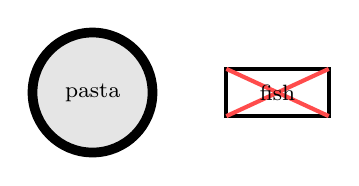
\begin{tikzpicture}
\draw[line width=3.5pt, fill=black!10] (-1.5,0) circle (0.3in);
\node at (-1.5,0) {\footnotesize pasta};
\draw[line width=1.5pt] (0.2,-0.3) rectangle (1.5,0.3);
\draw[line width=1.5pt, red!70] (0.2,-0.3) -- (1.5,0.3);
\draw[line width=1.5pt, red!70] (0.2,0.3) -- (1.5,-0.3);
\node at (0.85,0) {\footnotesize fish};
\end{tikzpicture}
\end{center}

This curriculum calls this deliberate act of deciding against an option, on purpose, a \textbf{Refuse}. A Refuse is not silence. It is not simply skipping past something without mentioning it. It is an active decision, just as real and just as worth recording as a Pop, that says: this one, specifically, not this time.

\begin{algorithmproc}{Is This a Refuse?}
Ask two questions. First, was this option genuinely available and considered, not simply absent from the situation altogether? Second, was a deliberate decision made against it, rather than it just happening to go unmentioned? If both answers are yes, you have found a Refuse, not merely an absence.
\end{algorithmproc}

\begin{practicenow}
Think of a recent choice you made among at least two options where you can clearly remember considering, and then rejecting, one specific alternative. Describe what made that a deliberate refusal rather than simply not thinking of it.
\end{practicenow}

\begin{exercisebox}{Section 1.1}
\item A voter reads all the candidates on a ballot and marks one of them, leaving the others unmarked. Are the unmarked candidates ``refused,'' in the sense of this workbook, or simply not chosen? Explain your reasoning.
\item Describe the difference between a friend who was never invited to a party and a friend who was invited but declined.
\item Challenge: can ``never considering'' an option ever later turn into ``refusing'' it, once you do consider it and decide against it? Explain using an example.
\end{exercisebox}

\chapter{Refused Is Not the Same as Gone}

\section{Two Very Different Kinds of ``No Longer There''}

This is the central idea of the whole workbook, and it deserves to be stated as plainly as possible: something can be genuinely refused, and still be entirely present, visible, and available to look at.

Compare two situations. In the first, a library never received a particular book request at all, so there is nothing on file anywhere, no record, no trace. In the second, a librarian receives the request, considers it, and decides to decline it, but keeps a note: request received, declined, for this reason. In both cases, you do not end up with the book. But the two situations are not remotely the same. In the second, there is a complete, checkable record of what happened. In the first, there is nothing to check at all, because nothing was ever recorded to begin with.

\begin{center}
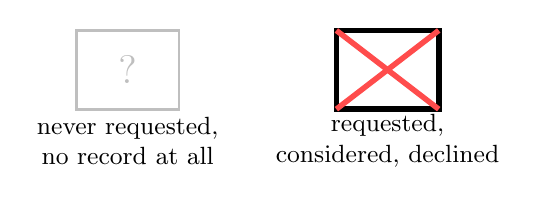
\begin{tikzpicture}
\draw[line width=1pt, gray!50] (-2.3,-0.5) rectangle (-1,0.5);
\node[gray!50] at (-1.65,0) {\Large ?};
\node[align=center, font=\small] at (-1.65,-0.9) {never requested,\\no record at all};
\draw[line width=2pt] (1,-0.5) rectangle (2.3,0.5);
\draw[line width=2pt, red!70] (1,-0.5) -- (2.3,0.5);
\draw[line width=2pt, red!70] (1,0.5) -- (2.3,-0.5);
\node[align=center, font=\small] at (1.65,-0.9) {requested,\\considered, declined};
\end{tikzpicture}
\end{center}

\begin{algorithmproc}{Absence Versus Refusal}
If you cannot point to a specific moment when something was considered and decided against, you are looking at an absence, not a refusal. If you can point to that moment, and to a reason or at least a record that it happened, you are looking at a refusal. The test is whether there is something to check, not merely whether the outcome, no result, looks the same either way.
\end{algorithmproc}

\begin{trythis}
Think of a real example of each: something that was genuinely never considered by anyone (an absence), and something that was considered and specifically turned down (a refusal). Write both down, and explain what evidence would let someone else tell them apart.
\end{trythis}

\begin{exercisebox}{Section 2.1}
\item A scientist runs an experiment and rules out one possible explanation based on the data, writing down exactly why. A different explanation is never even considered because nobody thought of it. Explain which of these is a refusal and which is an absence, in the sense of this workbook.
\item Describe a situation in your own life where keeping a record of something you decided against turned out to be useful later.
\item Challenge: is it possible to refuse something and later change your mind and choose it after all? What would that require, given that a refusal is supposed to be a real, recorded event?
\end{exercisebox}

\chapter{Why Keep a Record of What Didn't Happen}

\section{The Value of Knowing What Was Ruled Out}

It might seem strange to spend effort recording something that did not happen. Here is why it matters. A jury that hears a piece of evidence and is instructed to disregard it is in a very different position from a jury that never heard that evidence at all, even though the jury's final decision might not mention that evidence either way. Knowing that something was considered and specifically excluded, rather than simply never encountered, can change how much you trust a final decision, and can matter enormously if that decision is ever questioned later.

The same is true in much smaller, everyday situations. If you are trying to fix something that is broken, and you keep a written note of each possible cause you checked and ruled out, you save yourself and anyone helping you from checking the same dead end twice. Without that record, ruling something out is easy to forget, and the same wrong guess can get tried again and again.

\begin{summarybox}
A Refuse is a deliberate decision against a specific, considered option, and it leaves behind a permanent, checkable record, unlike a simple absence, where an option was never considered at all. Refused is not the same as gone: a refused option remains visible, nameable, and available to point to, exactly as much as a chosen one, differing only in which one was selected this time.
\end{summarybox}

\begin{exercisebox}{Section 3.1}
\item Describe a real situation where knowing something was ``tried and ruled out'' rather than ``never tried'' would change how you approached a problem.
\item Explain in your own words why a jury instructed to disregard evidence is in a meaningfully different position from a jury that never heard it, even if their final verdict looks the same either way.
\item Challenge: can you think of a situation where keeping a record of a refusal could cause a problem, rather than helping? What would make refusal-keeping risky or unwanted in that case?
\end{exercisebox}

\chapter*{Looking Ahead}
\addcontentsline{toc}{chapter}{Looking Ahead}

This workbook has treated Pop and Refuse as two separate, independent kinds of events. But could a Pop and a Refuse, or two Pops, be connected to each other on purpose, so that one depends on the other without the two becoming the same thing? That is the subject of the next workbook, Sproll 05: Together.

\chapter*{For Parents and Teachers}
\addcontentsline{toc}{chapter}{For Parents and Teachers}

This workbook introduces Refuse, the second of the four primitive actions this curriculum is built from. The distinction it insists on, between a deliberate, recorded refusal and a mere absence, is not a simplification; it is the exact formal content of the claim, elsewhere in this curriculum's technical material, that refusing an option documents its inadmissibility without removing it from the record of what remains historically nameable. A much later workbook in this series returns to this same distinction at a considerably higher level of precision, contrasting a refused option with two further, formally distinct ways an option can lose standing, so it is worth this workbook's care in getting the basic version right the first time.

\end{document}
